\documentclass[a4paper,12pt]{article}
\usepackage[utf8x]{inputenc}
\usepackage [T1]{fontenc}
\usepackage{datetime}
\usepackage{indentfirst}
\usepackage{float}
\usepackage{subcaption}
\captionsetup{compatibility=false}
\usepackage[T2A]{fontenc}
\usepackage[hmargin={20mm,10mm},vmargin={20mm,15mm},bindingoffset=0mm]{geometry}
\usepackage[colorlinks=true, linkcolor=black, citecolor=blue, urlcolor=blue, unicode]{hyperref}
\usepackage{docstyle}

\begin{document}
\begin{titlepage}
	\centering
	{\scshape\large VILNIAUS UNIVERSITETAS \\
	MATEMATIKOS IR INFORMATIKOS FAKULTETAS \par}
	\vspace{6cm}
	{\huge\bfseries Kompiuterinė rega. Teksto atpažinimas\par}
	{\LARGE Tiriamojo seminaro ataskaita\par}
	{\Large Matematinė informatika 3 kursas}
	\vspace{3cm}
	\vfill
	\flushright
	Autorius: \\ Ignas Jatulis\par
	\vspace{0.5cm}
	Vadovas: \\ Irus Grinis
	\vfill
	\centering
	Vilnius\\
	{\the\year}
\end{titlepage}	
\tableofcontents

\newpage
\section*{Įvadas}
\addcontentsline{toc}{section}{Įvadas}

Šiais laikais žmonės vis daugiau veiksmų atlieka kompiuterio pagalba. Pavyzdžiui, jei seniau studentai sesijos metu, prieš egzaminus, konsektus rašydavo ranka, tai šiais laikais, vis daugiau studentų renkasi kompiuterį, jame esančias teksto rengykles, kurių pagalba galima patogiai ir tvarkingai parengti konspektus. Tačiau sudarydami konspektus iš ranką rašytų sąsiuvinių, jie sugaišta nemažai laiko.  Tad kodėl nesukūrus kompiuterinės programos ar mobiliosios programėlės, kurios pagalba užtektų nufotografuoti ar nuskenuoti tekstą, o kompiuteris jį pats atpažintų? \\
\indent Taigi, šio darbo galutinis tikslas - ranka rašyto teksto atpažinimo programėlė. Šiam tikslui pasiekti, pasitelksime vieną populiariausių kompiuterinės regos bibliotekų OpenCV ir sukonstruotą dirbtinį neuronų tinklą.

\newpage
\section{OpenCV biblioteka}
Nuotraukų apdorojimui buvo pasirinkta OpenCV biblioteka  (\cite{OpenCVabout}). OpenCV (Open Source Computer Vision Library) yra atvirojo kodo kompiuterinės regos biblioteka. Šią biblioteką galima naudoti tiek mokslo, tiek komercijos tikslais.\\
\indent Šioje kompiuterinės regos bibliotekoje yra realizuota daugiau kaip 2500 optimizuotų algoritmų kurie padeda apdirbti vaizdus. Taip pat ji pritaikyta programuoti su tokiomis kalbomis kaip C++, C, Python, JAVA ir yra suderinama su populiariausiomis operacinėmis sistemomis, tokiomis kaip Windows, Linux, Android ar Mac OS. Apie kiekvieną bibliotekoje esantį algoritmai ir jo panaudojimo pavyzdžius, galima rasti OpenCV dokumentacijoje  (\cite{OpenCVdoc}).

\section{Nuotraukų apdorojimas teksto atpažinimui}
Kad kompiuteris tiksliau atpažintų tektą, visų pirma reikalingas to paveiksliuko apdorojimas. Apdorojimas susideda iš  (\cite{KavaliauskasFelinskas, Beigi}):
\begin{itemize}
	\item nuotraukos nuskaitymas;
	\item nuotrauką paverčiame į nespalvotą (pilką);
	\item apdorojame nuotrauką slenkčių (thresholding) algoritmais, t.y. paverčiama tik į juodai baltą;
	\item teksto atvaizdą išvalome nuo „triukšmo“ - pašaliname atsitiktinius pikselius, kurie galėjo atsirasti skenuojant ar fotografuoajnt tekstą;
	\item atliekame vaizdo aštinimo procedūras, kurios padės išryškinti teksto kontūrus;
	\item atliekame teksto ploninimą;
\end{itemize}
Šio apdorojimo paskirtis yra palengvinti atpažinimą ir sumažinti duomenų kiekį, kurį turės apdoroti teksto atpažinimo algoritmas.
\section{Segmentacija}
Didžiausia probleminė sritis norint atpažinti tekstą, yra teksto segmentaciją iš nuotraukos. Nuo to priklauso, ar teisingai bus atskirti žodžiai ir simboliai teisingam teksto atpažinimui. Tai atliekant kyla nemažai iššūkių, tokių kaip: 
\begin{itemize}
	\item teksto eilutės išskyrimas;
	\item žodžio atskirimas iš eilutės;
	\item žodžio segmentacija į raides;
\end{itemize}
\indent Skaidant į teksto eilutes  problema atsiranda tuomet, kai teksta parašytas netolygiai, t.y. viena eilutė gali pakilti ar nusileisti ir taip patekti į kitos eilutės rėžius. \\
\indent Skaidant gautas eilutės į žodžius problema atsiranda tuomet, kai to paties žodžio raidės nėra visos tarpūsavyje sujungtos. Kad to išvengti, tekstą papildomai apdoroju išliejimo (angl. blur) funkcija, kad „užlopyti“ smulkius tarpus.\\
\indent Ir galiausiai, gautus žodžius segmentuojant į raides, problema atsiranda tuomet, kai raidės yra sujungtos. Kadangi bandoma raides atskirti tose vietose, kur linija tampa ploniausia, tai nebūtinai reiškia, kad būtent toje vietoje ir jungiasi žodžiai. Pavyzdžiui bandant atskirti raidę `u' neretai ją perskeldavo pusiau.

\newpage
\section{Pavyzdys}
Turime nuotrauką, kurioje yra nufotografuoti žodžiai parašyti ant popieriaus lapo.
\begin{center}
	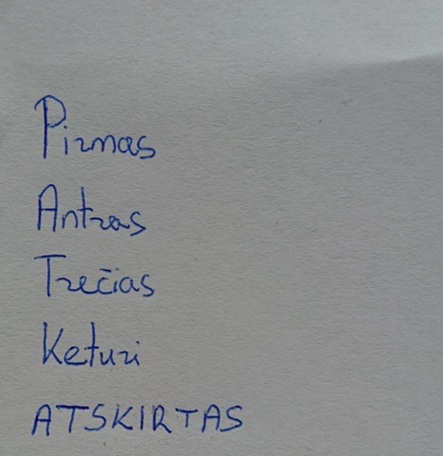
\includegraphics[scale=0.75]{img/1.png}\\
	\textbf{Pav. 1}: Nufotografuotas tekstas\\
\end{center}

Pasileidžiame programą:\\
\verb|java -jar -Djava.library.path=C:\opencv3.2\build\java\x64 TextRecognition.jar|
ir pasirenkame  „Iškirpti žodžius“ meniu punktą.

\begin{center}
	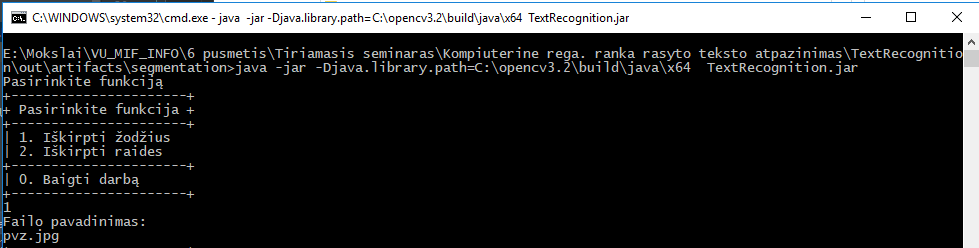
\includegraphics[scale=0.7]{img/2.png}\\
	\textbf{Pav. 2}: Pasirenkame meniu punktą\\
\end{center}
Suvedus nuotrauko failo pavadinimą, procedūra apdoroja paveiksliuką ir aplanke words sukuria naujus paveiksliukus, kuriuose po vieną žodį.
 
\begin{figure}[H]
\centering
\begin{subfigure}{.5\textwidth}
  \centering
  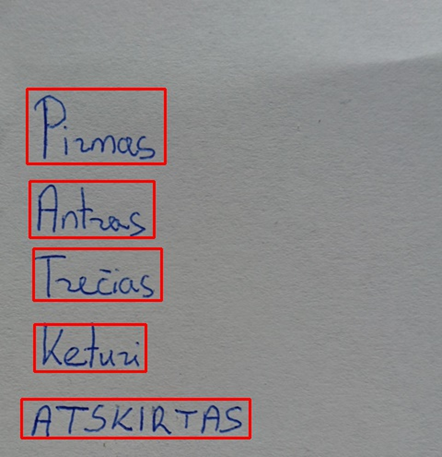
\includegraphics[height=.9\linewidth]{img/3.1.png}
  \caption{Programa atpažįsta konturus tų vietų, kuriuose yra žodžiai}
\end{subfigure}%
\begin{subfigure}{.5\textwidth}
  \centering
  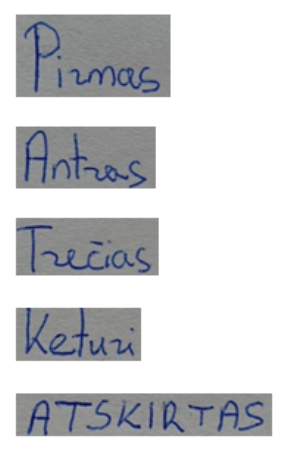
\includegraphics[height=.9\linewidth]{img/3.2.png}
  \caption{Kiekvienas kontūras iškerpamas ir išsaugomas į atskirą failą}
\end{subfigure}
\textbf{Pav 3}. Žodžių atpažinimas paveiksliuke ir iškarpymas.\\
\end{figure}

Paskui pasirinkę naujai iškirpto žodžio failą bei meniu punktą „Iškirpti raides“ gauname rezultą. 

\begin{center}
	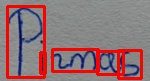
\includegraphics[scale=0.7]{img/4.jpg}\\
	\textbf{Pav. 4}: Pasirenkame raidžių segmentavimą\\
\end{center}

Kas yra apibrauktą raudonais keturkampiais bus išsaugota letters aplanke. Tai bus medžiaga, kurią bandys atpažinti sekančiame semestre sukurtas neuroninis tinklas.

\clearpage
\section*{Išvados}
\addcontentsline{toc}{section}{Išvados}
Taigi, per šį semestrą buvo atliktas žodžių segmentavimas iš nuotraukų. Nuotraukoje esantys žodžiai išsaugomi kaip atskiri *.jpg formato paveiksliukai. Taip pat buvo bandoma, kuo optimaliau atlikti žodžių segmentaciją į raides. Jei žodžio raidės nėra sujungiamos, tai raides susegmentuodavo beveik 100\% tikslumu. Didžioji problema yra žodžio skaidymas, kai raidės yra sujungtos. Buvo bandoma spėti, jog vieta, per kurią reiktų skelti paveiksliuką ir jog tai raidžių susijungimo vieta yra toje vietoje, kur linija jungianti raides įgyja mažiausią reikšmę, tai yra, ten, kur raides jungianti linija yra ploniausia. Atlikus testus paaiškėjo, jog toks segmentavimas efektingas tik apie 50 \% atvejų.\\
\indent Sekančiame semestre bus siekiama dar labiau patobulinti segmentavimo į raides algoritmą ir sukurti kelių sluoksnių neuroninį tinklą bei apmokyti kompiuterį atpažinti pateiktas raides.

\newpage
\renewcommand{\refname}{Literatūra}
\addcontentsline{toc}{section}{Literatūra}
\begin{thebibliography}{99}

\bibitem {OpenCVdoc}
OpenCV documentacija. 
\url{http://docs.opencv.org/}

\bibitem {OpenCVabout}
Apie OpenCV.
\url{http://opencv.org/about.html}
[Žiūrėta 2017 m. gegužės mėn.]

\bibitem {KavaliauskasFelinskas}
G.  Kavaliauskas, G. Felinskas. Dirbtinio intelekto atpažinimo metodų analizė ir taikymai ranka rašytam tekstui atpažinti. Jaunųjų mokslininkų darbai  (Nr. 4(37)), 2012, p. 205-211

\bibitem {Beigi}
H.S.M. Beigi.  An overview of handwriting recognition. Proceedings of the 1 st Annual Conference on Technological Advancements in Developing Countries, 1993, p. 30-46

\end{thebibliography}

\end{document}

